\chapter{Генерация синтетических данных для обучения}

\section{Мотивировка использования синтетических данных}

Современные методы обучения с использованием нейросетей требуют значительного
объёма размеченных данных для достижения удовлетворительной точности. Однако
традиционные наборы данных, размеченные вручную, имеют ряд ограничений, особенно
в прикладных инженерных задачах.

\begin{enumerate}
  \item Ручная аннотация даже тысячи изображений требует сотен часов
  человеческого труда, а также подвержена ошибкам, связанным с субъективностью
  разметчика и человеческим фактором.
  \item Стандартные открытые наборы данных, например, для сегментации
  используют COCO\footnote{\url{https://cocodataset.org/}} или
  OpenImages\footnote{\url{https://storage.googleapis.com/openimages/web/index.html}},
  для задач MVS — ShapeNet\footnote{\url{https://shapenet.org/}},
  ABC\footnote{\url{https://deep-geometry.github.io/abc-dataset/}},
  BlendedMVS\footnote{\url{https://github.com/YoYo000/BlendedMVS}},
  DTU\footnote{\url{https://roboimagedata.compute.dtu.dk/}} и другие, не
  содержат узкоспециализированных объектов, необходимых для задач, связанных с
  прозрачными или оптически сложными материалами, такими как стекло или
  драгоценные камни. В большинстве случаев они ориентированы на распознавание
  предметов общего назначения (мебель, бытовая техника и т.п.).
  \item Такие наборы, как правило, не включают точные аннотации глубины,
  параметров камеры или тепловых карт, которые необходимы для задач трёхмерной
  реконструкции и требуют использования дополнительных дорогостоящих сенсоров
  или ручной постобработки.
  \item Наконец, даже при наличии подходящего набора данных, нельзя полагаться
  на постоянный доступ к нему: он может оказаться временно недоступным из-за
  технических сбоев, изменения политики распространения, либо ограничения
  доступа по регионам. Таким образом, отсутствие локальной копии делает
  невозможным воспроизведение эксперимента в любой момент.
\end{enumerate}

Использование синтетических наборов данных позволяет преодолеть
вышеперечисленные ограничения:
\begin{enumerate}
  \item Генерация разметки может быть полностью автоматизирована и выполнена с
  абсолютной точностью: можно получать точные пиксельные маски, карты глубины,
  нормали, координаты ключевых точек, параметры освещения и позы камеры.
  \item Состав сцены и объектов может быть произвольно задан пользователем,
  включая модели, не существующие в реальности, что особенно полезно при
  исследовании теоретических или проектируемых объектов.
  \item В случае ограниченного или нестабильного доступа к интернету
  синтетические данные, созданные локально, обеспечивают независимость от
  внешних хранилищ и повышают воспроизводимость экспериментов.
\end{enumerate}

Таким образом, синтетические данные становятся не просто заменой, а зачастую
необходимым условием для воспроизводимого и точного эксперимента в задачах,
выходящих за рамки типовых сценариев компьютерного зрения.

\section{Выбор инструмента для генерации синтетических данных}

Для получения качественных синтетических изображений с аннотациями глубины,
масок, траекторий камер и прочих параметров требуется инструмент, одновременно
обеспечивающий физически корректный рендеринг, полную управляемость сцены и
возможность масштабируемой автоматизации. Среди всех доступных решений
оптимальным выбором в рамках данной работы является программа
Blender\footnote{\url{https://www.blender.org/}}.

Одним из ключевых преимуществ Blender является его \emph{свободное распространение}:
программа имеет открытую лицензию и полностью бесплатна. Это отличает её от
коммерческих пакетов, таких как Autodesk
Maya\footnote{\url{https://www.autodesk.com/products/maya/overview}}, 3ds
Max\footnote{\url{https://www.autodesk.com/products/3ds-max/overview}} или
рендеринговых движков вроде V-Ray\footnote{\url{https://www.chaos.com/vray}},
лицензии на которые могут стоить значительные суммы.  Открытый исходный код
Blender также означает, что пользователь может детально изучить поведение
системы и при необходимости модифицировать её под собственные задачи.

Вторым важным достоинством является \emph{унификация рабочего процесса}. В одной
программе объединены средства трёхмерного моделирования, система настройки
материалов по физически корректной модели отражения (в частности, поддержка
шейдера Principled
BSDF\footnote{\url{https://docs.blender.org/manual/en/latest/render/shader_nodes/shader/principled.html}}),
средства высокоточного рендеринга с использованием трассировки лучей (движок
Cycles\footnote{\url{https://docs.blender.org/manual/en/latest/render/cycles/index.html}}),
а также возможность быстрого предварительного просмотра сцены (движок
Eevee\footnote{\url{https://docs.blender.org/manual/en/latest/render/eevee/index.html}}).
Это позволяет не переключаться между разными приложениями при подготовке,
проверке и генерации изображений.

Третьим и, пожалуй, наиболее значимым фактором является \emph{автоматизация}.
Все действия, доступные в графическом интерфейсе Blender, могут быть
воспроизведены программно с использованием встроенного языка
Python\footnote{\url{https://www.python.org/}}. Это даёт возможность создавать
сцены, управлять положением камер, освещением и материалами, а также производить
рендеринг и экспорт аннотаций полностью автоматически, в пакетном режиме, в том
числе и на сервере без графического интерфейса (режим ``без головы'', англ.
headless). Такая гибкость делает Blender исключительно подходящим для генерации
больших объёмов данных с заданной структурой и повторяемостью.

Наконец, Blender — это кроссплатформенное решение, доступное для операционных
систем Windows, Linux и macOS. Проект поддерживается сообществом и развиваем при
участии ведущих технологических компаний, что обеспечивает устойчивое развитие и
быстрое внедрение современных графических технологий.

Альтернативные решения, доступные на рынке, в сравнении с Blender имеют
существенные ограничения. Так, игровые движки, такие как
Unity\footnote{\url{https://unity.com/}} или Unreal
Engine\footnote{\url{https://www.unrealengine.com/en-US}}, избыточны по
возможностям при решении задач генерации статичных изображений. Они часто
сопровождаются сложными условиями лицензирования и могут требовать платных
подписок или предварительного коммерческого согласования.  Более того, их
архитектура ориентирована в первую очередь на интерактивные сцены, а не на
контроль точности визуализации.

Есть и специализированные инструменты, такие как
UnrealCV\footnote{\url{https://unrealcv.org/}},
SynthEyes\footnote{\url{https://borisfx.com/products/syntheyes/}} или другие
пакеты для визуального трекинга и аннотирования. Однако большинство из них либо
ограничены по функциональности (например, работают только с одной моделью
камеры), либо сложны в интеграции и настройке.

Таким образом, Blender в силу своей универсальности, автоматизируемости,
доступности и поддержки профессионального рендеринга представляет собой наиболее
рациональный выбор для создания синтетических наборов данных в рамках задачи
реконструкции построения сложных геометрических фигур.

\section{Автоматизация синтетической генерации датасетов}

\subsubsection{Постановка задачи}
Необходимо разработать и реализовать с использованием Blender Python API программу (скрипт),
автоматически генерирующую синтетические изображения заданной 3D-модели.
Полученные рендеры должны сопровождаться полной аннотацией: маски, глубина,
нормали, параметры камеры, положение источников света. Результирующий датасет
предназначен для обучения и валидации алгоритмов многовидовой
стереореконструкции и нейросетевых моделей восстановления 3D (NeRF, MVS и др.).

\noindent Скрипт должен выполнять следующие действия:
\begin{enumerate}
  \item Получить от клиента путь до 3D-модели, путь до желаемой папки с
  результатами и желаемое количество элементов в датасете.
  \item Загрузить 3D-модель в форматах OBJ, FBX или glTF/GLB, расположенную по пути клиента.
  \item Дать возможность с помощью внешнего конфигурационного файла настроить
  мир, фон, разрешение итоговой картинки, движок для рендеринга и параметры к
  нему.
  \item Организовать программно равномерное освещение импортированного объекта.
  \item Запустить цикл по количеству желаемых элементов:
  \begin{enumerate}
    \item Добавить камеру с настраиваемыми параметрами линзы, сенсора и
    глубины резкости (англ. Depth of field , DOF).
    \item Для каждого кадра случайно выбирать точку на верхней полусфере и
    направлять камеру в центр сцены.
    \item Предоставить возможность клиенту получить доступ к сцене, миру и
    камере для получения параметров камеры или генерации глубины.
    \item Запустить рендер, сохранить файл в результирующую папку.
  \end{enumerate}
\end{enumerate}

\subsubsection{Результаты выполнения задачи}

Скрипт использует программу Blender без загрузки пользовательского интерфейса, то
есть в ``безголовом режиме'' (\texttt{blender -{}-background}) и принимает три
позиционных аргумента: путь к 3D-модели, директорию для вывода и требуемое число
кадров. Все числовые и логические настройки считываются из конфигурационного
файла, поэтому изменение качества рендера, размеров кадра или схемы освещения не
требует изменений в коде.

После предварительной очистки сцены импортируется файл соответствующего
расширения (OBJ, FBX, glTF/GLB). Предполагается подготовительная обработка
модели: нужно убедиться центрирован ли объект, убрать возможные помехи.

Освещение сцены можно настроить несколькими способами. Есть возможность использовать
равномерное распределение источников света вокруг объекта. Другой способ — задействовать
текстуры окружения (англ. Environment textures), тем самым получить реалистичное освещение.

Камера формируется на каждом кадре заново. Положение камеры задается случайной
точкой на верхней полусфере, диапазоны для радиуса, склонения и азимута также
конфигурируемы. Камера смотрит в центр. При включённой глубине резкости
автоматически высчитывается дистанция фокуса.

Структура плагинов (англ. plugins) позволяет расширить возможности приложения,
не меняя исходный код основной части. Скрипт динамически импортирует все подпакеты
из директории \texttt{plugins}, регистрирует их и вызывает подпрограммы пользователя
в заданных местах, тем самым предоставляя возможность получить доступ к сцене и камере.

Различные примеры запуска, исходный код, полезные ссылки на документацию можно найти
по ссылке \url{https://github.com/SherAndrei/blender-gen-dataset}.

\subsubsection*{Используемые библиотеки}

\begin{itemize}
    \item \texttt{bpy} и \texttt{mathutils} — встроенные модули Blender;
    \item \texttt{argparse}, \texttt{random}, \texttt{importlib},
    \texttt{shutil}, \texttt{os} — стандартный Python без внешних зависимостей.
    \item \texttt{tomllib} — с Python 3.11 это часть стандартной библиотеки;
    TOML\footnote{\url{https://toml.io/en/}} выбран за простоту чтения человеком
    и хорошую типизацию.
\end{itemize}

Иных пакетов нет: скрипт собирается и работает ``из коробки'' внутри
официального дистрибутива Blender.

\begin{figure}[t]
\begin{minipage}{0.5\linewidth}
	\centering
	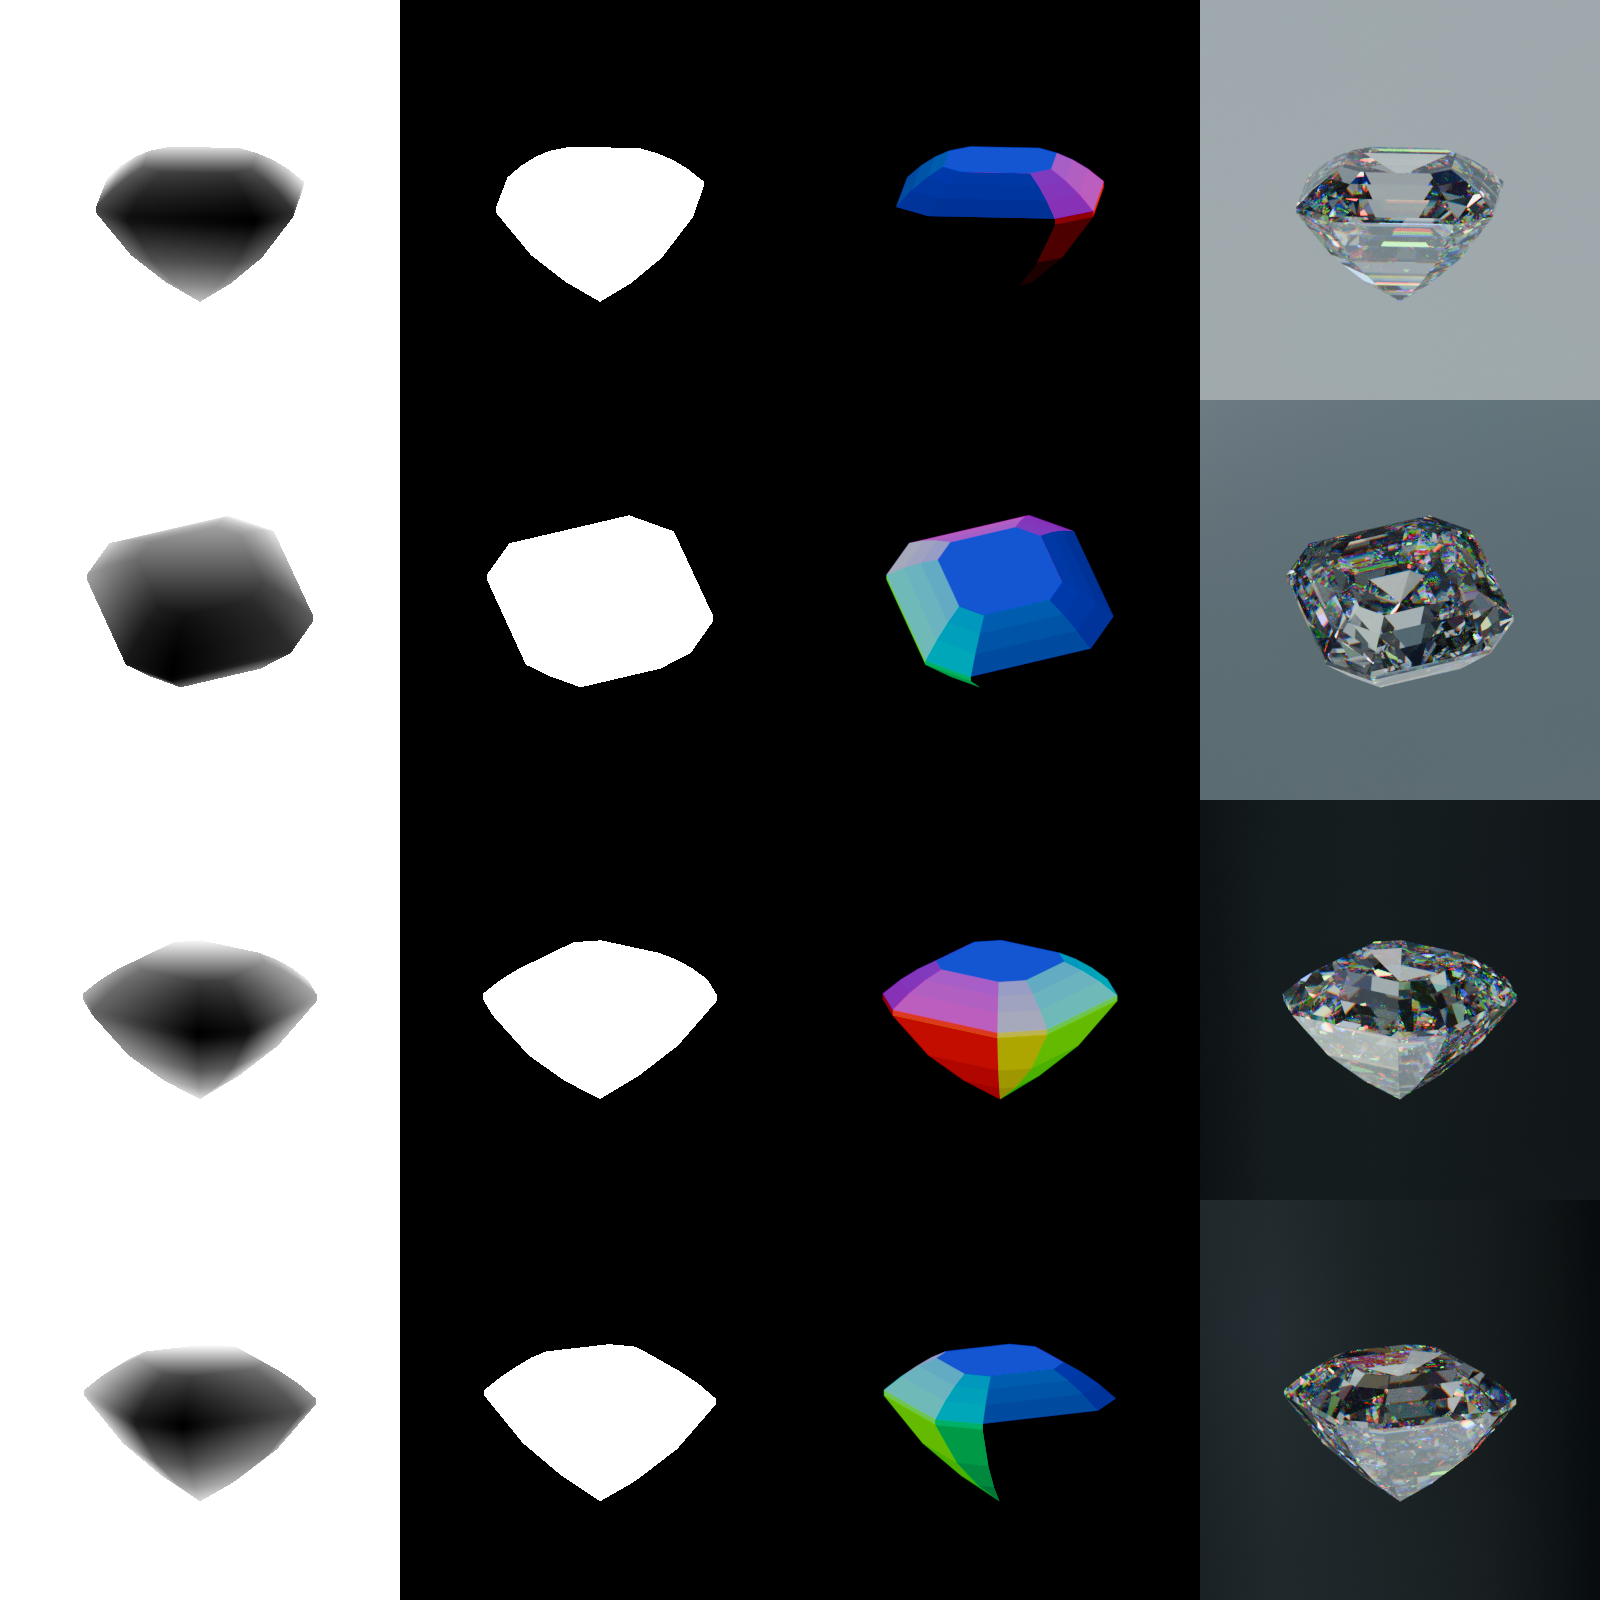
\includegraphics[scale=0.1]{assher.png}
	\caption{Бриллиант Asscher}
\end{minipage}%
\begin{minipage}{0.5\linewidth}
	\centering
	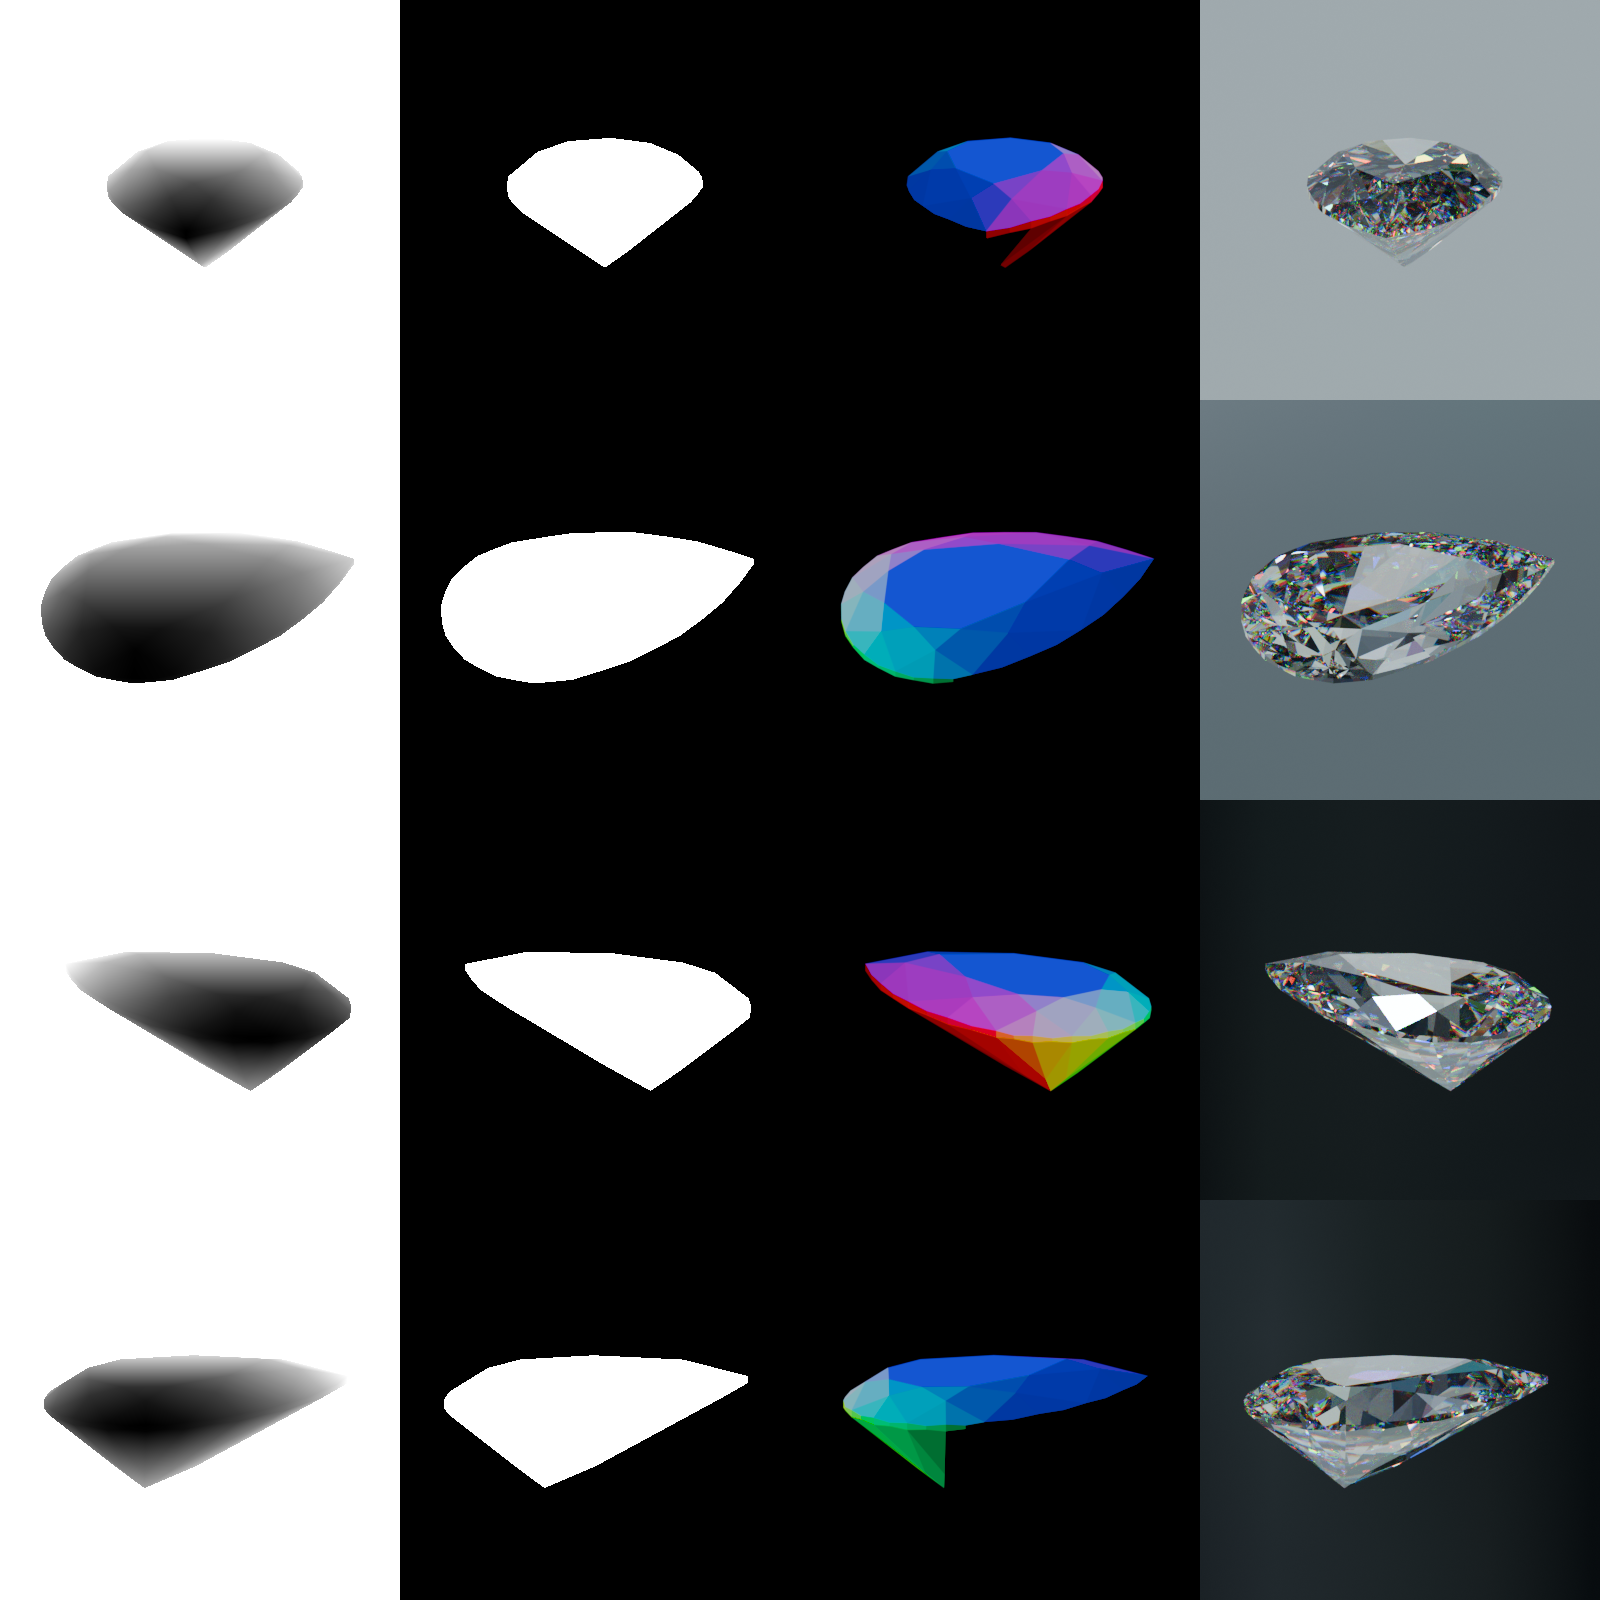
\includegraphics[scale=0.1]{pear.png}
	\caption{Бриллиант Pear}
\end{minipage}

\vspace{0.4cm}

\begin{minipage}{0.5\linewidth}
	\centering
	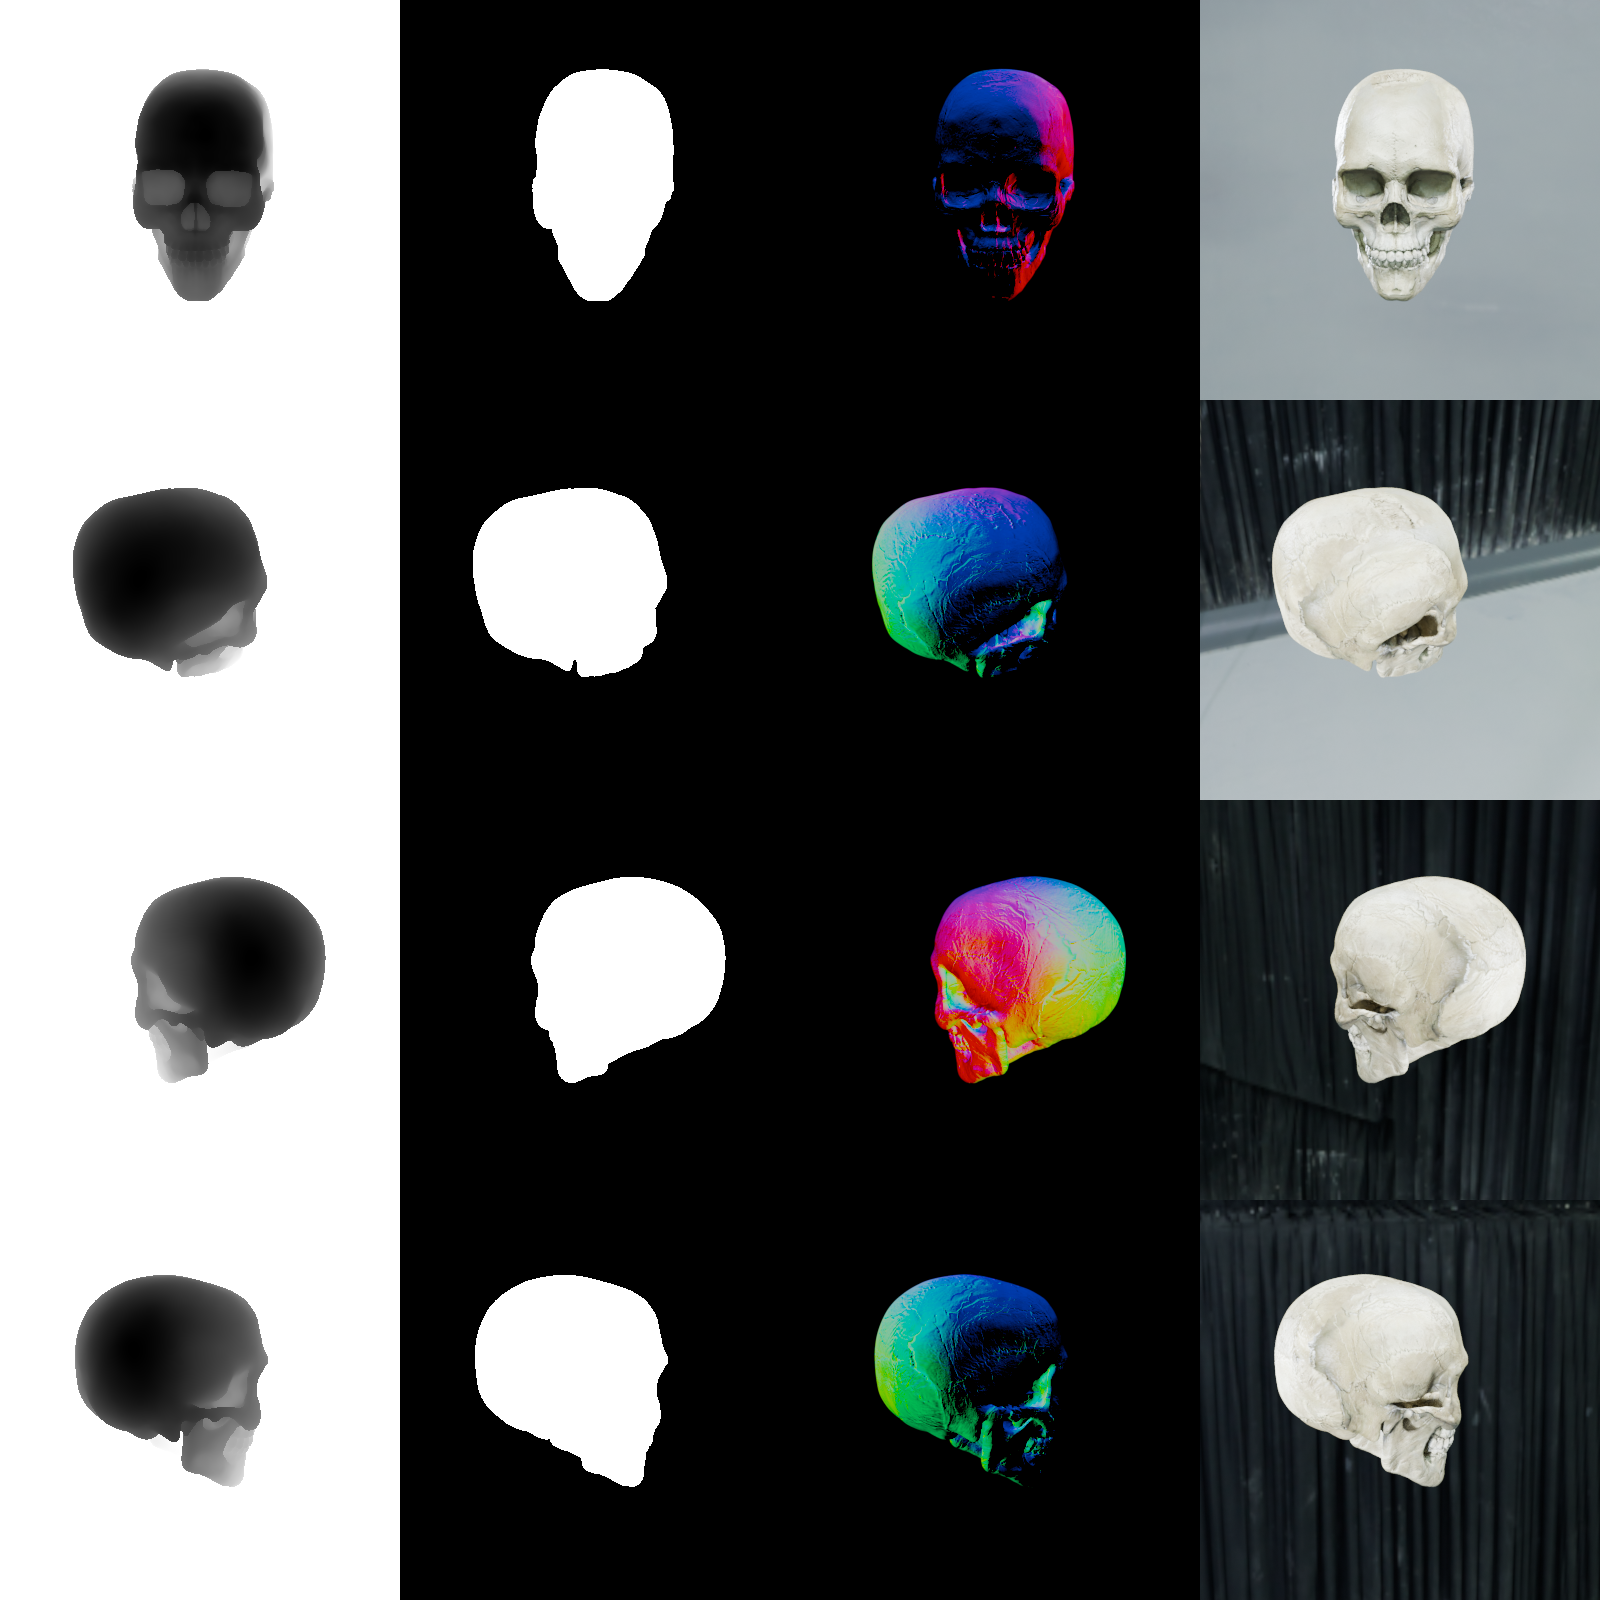
\includegraphics[scale=0.1]{female.png}
	\caption{Женский череп}
\end{minipage}%
\begin{minipage}{0.5\linewidth}
	\centering
	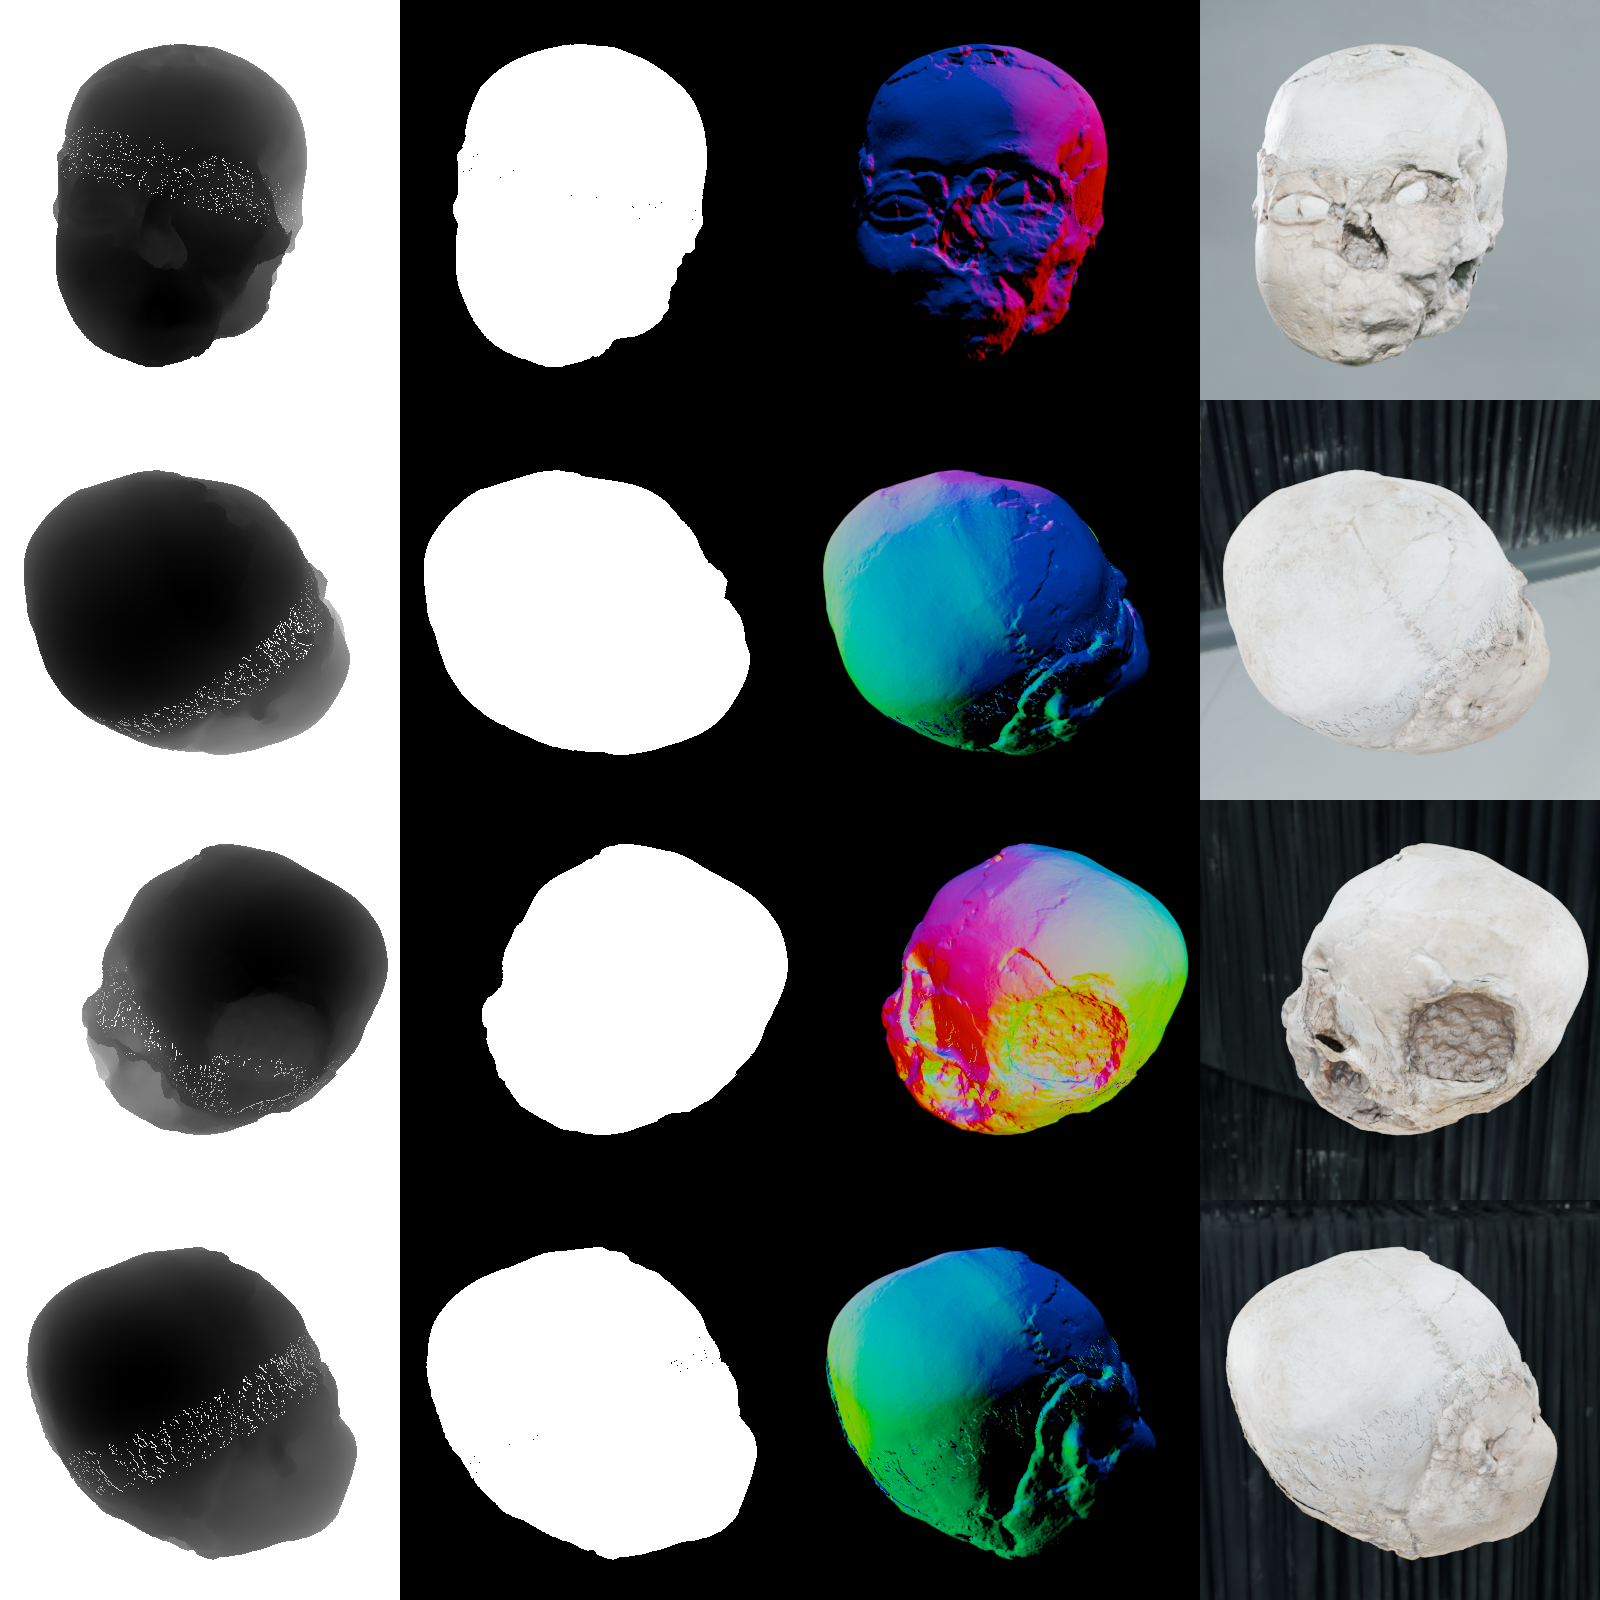
\includegraphics[scale=0.1]{jericho.png}
	\caption{Череп жителя Йерихона}
\end{minipage}
\end{figure}

\subsubsection*{Условия проведения экспериментов и используемые ресурсы}

Для решения поставленной задачи в данной работе были использованы 3D-модели
драгоценных камней и черепов, найденные на платформах BlenderKit
\footnote{\url{https://www.blenderkit.com/terms-and-conditions-2021/}} и Sketchfab
\footnote{\url{https://sketchfab.com/feed}}. Текстуры окружения, необходимые для создания
реалистичных сцен, были загружены с ресурса Poly Haven
\footnote{\url{https://polyhaven.com/hdris}}.

Генерация синтетических датасетов выполнялась в Blender 4.2.9 LTS (сборка от
15.04.2025) с использованием встроенного интерпретатора Python 3.11.7.

Эксперименты проводились на персональном ноутбуке с конфигурацией: ОС: Windows
11 Home (версия 10.0.22631, сборка 22631); процессор: AMD Ryzen 5 4500U с
графикой Radeon (6 ядер, 2,38 ГГц); ОЗУ: 8 ГБ (7,42 ГБ доступно); графика:
интегрированная AMD Radeon.

Для генерации каждого набора из примера, а именно изображений в формате
\texttt{png} с разрешением 400 на 400, подсчета глубин, масок и нормалей,
понадобилось в среднем по одной минуте. Конфигурация позволила эффективно
генерировать синтетические датасеты, несмотря на ограниченные ресурсы мобильного
процессора и интегрированной графики.

\subsubsection*{Заключение}

Среди текущих ограничений стоит отметить необходимость ручной предобработки
некоторых моделей, что в перспективе можно автоматизировать средствами Blender
API. Отсутствие встроенной поддержки распределенного рендеринга по нескольким
графическим ускорителям компенсируется возможностью параллельного запуска
независимых экземпляров на разных компьютерах. Кроме того, разработка новых
плагинов требует определенного знания Blender API, хотя наличие базовых примеров
(таких как маски, глубины и нормали) существенно должно снизить порог входа.

Разработанный генератор синтетических данных представляет собой сбалансированное
решение, сочетающее простоту реализации с достаточной функциональностью для
исследовательских задач. Его ключевое преимущество заключается в декларативном
подходе - все параметры рендеринга, включая выбор движка для ренденринга,
задаются в конфигурационном файле, что обеспечивает прозрачность и простоту
настройки. Важной особенностью решения является гарантированная воспроизводимость
результатов благодаря поддержке seed-значений и детерминированных алгоритмов.
Это делает генератор особенно полезным для таких задач, как обучение NeRF,
тестирование MVS-алгоритмов или проверка исследовательских гипотез.
Несмотря на то, что решение не представляет собой готовую промышленную систему с
распределённой обработкой данных, его архитектура позволяет постепенно
наращивать функциональность, добавляя именно те компоненты, которые требуются в
конкретном проекте.
